% ---------------------------------------------------------------------------
% report.tex  --  ECE463 4-bit array multiplier, RTL to GDSII
% Build from this folder with:   tectonic report.tex
% ---------------------------------------------------------------------------
\documentclass[11pt,a4paper]{article}

\usepackage[margin=2.2cm]{geometry}
\usepackage{amsmath,amssymb}
\usepackage{booktabs}
\usepackage{tabularx}
\usepackage{array}
\usepackage{graphicx}
\usepackage{xcolor}
\usepackage{fancyvrb}
\usepackage{enumitem}
\usepackage{caption}
\usepackage{float}
\usepackage{tikz}
\usetikzlibrary{shapes.gates.logic.US, arrows.meta, calc}
\usepackage[hidelinks]{hyperref}

\setlength{\parindent}{0pt}
\setlength{\parskip}{5pt}
\setlist{itemsep=2pt, topsep=3pt}
\captionsetup{font=small, labelfont=bf}
\renewcommand{\arraystretch}{1.15}
\setlength{\emergencystretch}{3em}

\newcolumntype{Y}{>{\raggedright\arraybackslash}X}
\newcommand{\cell}[1]{\texttt{#1}}
\newcommand{\umsq}{\ensuremath{\mu\mathrm{m}^2}}
\newcommand{\um}{\ensuremath{\mu\mathrm{m}}}

\begin{document}

% ---------------------------------------------------------------------------
\begin{center}
  {\LARGE\bfseries 4-bit Array Multiplier: RTL to GDSII}\\[6pt]
  {\large ECE463 Digital VLSI Design \textbar{} Team Assignment Report}\\[12pt]
  \begin{tabular}{ll}
    Monishram Selvaraj & 2024102076 \\
    Neel Rajesh        & 2024102007
  \end{tabular}\\[8pt]
  Repository: \url{https://github.com/monishram2508/mult4-rtl-to-gds}\\[2pt]
  October 2026
\end{center}

\section{Summary}

A 4-bit unsigned array multiplier was written in Verilog, verified exhaustively,
synthesised to SkyWater SKY130 standard cells, timed with static timing analysis,
and taken through place and route to a DRC- and LVS-clean GDSII layout.

\begin{table}[H]
\centering
\begin{tabularx}{\textwidth}{lY}
\toprule
Part & Result \\
\midrule
A: RTL and verification & \texttt{PASS: 256 vectors checked, 0 errors} (RTL and gate-level netlist) \\
B: Logic synthesis      & 67 cells, of which 16 flip-flops; total area 746.97~\umsq{} \\
C: Static timing        & $T_{min} = 2.604$~ns, $F_{max} = 384.0$~MHz (typical corner) \\
D: Physical design      & First run passed at 3.5~ns: 0 DRC, 0 LVS, setup slack $+0.605$~ns, post-route $F_{max} = 345.4$~MHz \\
\bottomrule
\end{tabularx}
\end{table}

\textbf{Environment.} IIC-OSIC-TOOLS Docker image; PDK \texttt{sky130A}; standard
cell library \texttt{sky130\_fd\_sc\_hd}; typical corner \texttt{tt\_025C\_1v80}
for Parts B and C. Tools: Icarus Verilog and GTKWave (A), Yosys (B), OpenSTA (C),
LibreLane with OpenROAD, Magic, KLayout and Netgen (D). The exact command for
every step is listed in the repository README.

% ---------------------------------------------------------------------------
\section{Part A: RTL Design and Verification}

\subsection{Design}

\begin{table}[H]
\centering
\begin{tabular}{llll}
\toprule
Port & Direction & Width & Description \\
\midrule
\texttt{clk}   & input  & 1 & Clock, rising edge \\
\texttt{rst\_n} & input & 1 & Asynchronous reset, active low; clears all registers \\
\texttt{a}     & input  & 4 & Multiplicand \\
\texttt{b}     & input  & 4 & Multiplier \\
\texttt{p}     & output & 8 & Product $a \times b$, registered \\
\bottomrule
\end{tabular}
\end{table}

\texttt{rtl/mult\_array.v} has three layers:
\begin{enumerate}
  \item \textbf{Input registers.} \texttt{a} and \texttt{b} are captured into
        \texttt{a\_reg} and \texttt{b\_reg} (4 + 4 flip-flops) on every rising edge.
  \item \textbf{Combinational array,} built from the registered values: 16 AND
        gates form the partial products $pp_i[j] = a\_reg[j] \cdot b\_reg[i]$, and
        12 instances of \texttt{full\_adder} (\texttt{rtl/full\_adder.v}, written
        with \texttt{assign} statements) add them in three ripple-carry rows,
        instantiated with \texttt{generate} loops. The \texttt{*} operator is not used.
  \item \textbf{Output register.} The 8-bit result is captured into \texttt{p}
        (8 flip-flops).
\end{enumerate}
This gives exactly 16 flip-flops and a latency of 2 clock cycles: inputs are
captured at edge 1 and the product at edge 2. The array is wired exactly as the
connection table in Section 2 of the assignment:

\begin{table}[H]
\centering
\small
\begin{tabular}{lll}
\toprule
Row & Inputs to full adder $j$ ($j = 0\ldots3$) & Outputs \\
\midrule
0 & no adders & $p[0] = pp_0[0]$; \ $r_0 = \{0, pp_0[3], pp_0[2], pp_0[1]\}$ \\
1 & $pp_1[j]$, $r_0[j]$, $c_1[j]$ \ ($c_1[0] = 0$) & $p[1] = s_1[0]$; \ $r_1 = \{c_1[4], s_1[3], s_1[2], s_1[1]\}$ \\
2 & $pp_2[j]$, $r_1[j]$, $c_2[j]$ \ ($c_2[0] = 0$) & $p[2] = s_2[0]$; \ $r_2 = \{c_2[4], s_2[3], s_2[2], s_2[1]\}$ \\
3 & $pp_3[j]$, $r_2[j]$, $c_3[j]$ \ ($c_3[0] = 0$) & $p[3] = s_3[0]$; \ $p[7{:}4] = \{c_3[4], s_3[3], s_3[2], s_3[1]\}$ \\
\bottomrule
\end{tabular}
\end{table}

\subsection{Block diagram}

\begin{figure}[H]
\centering
\resizebox{\textwidth}{!}{%
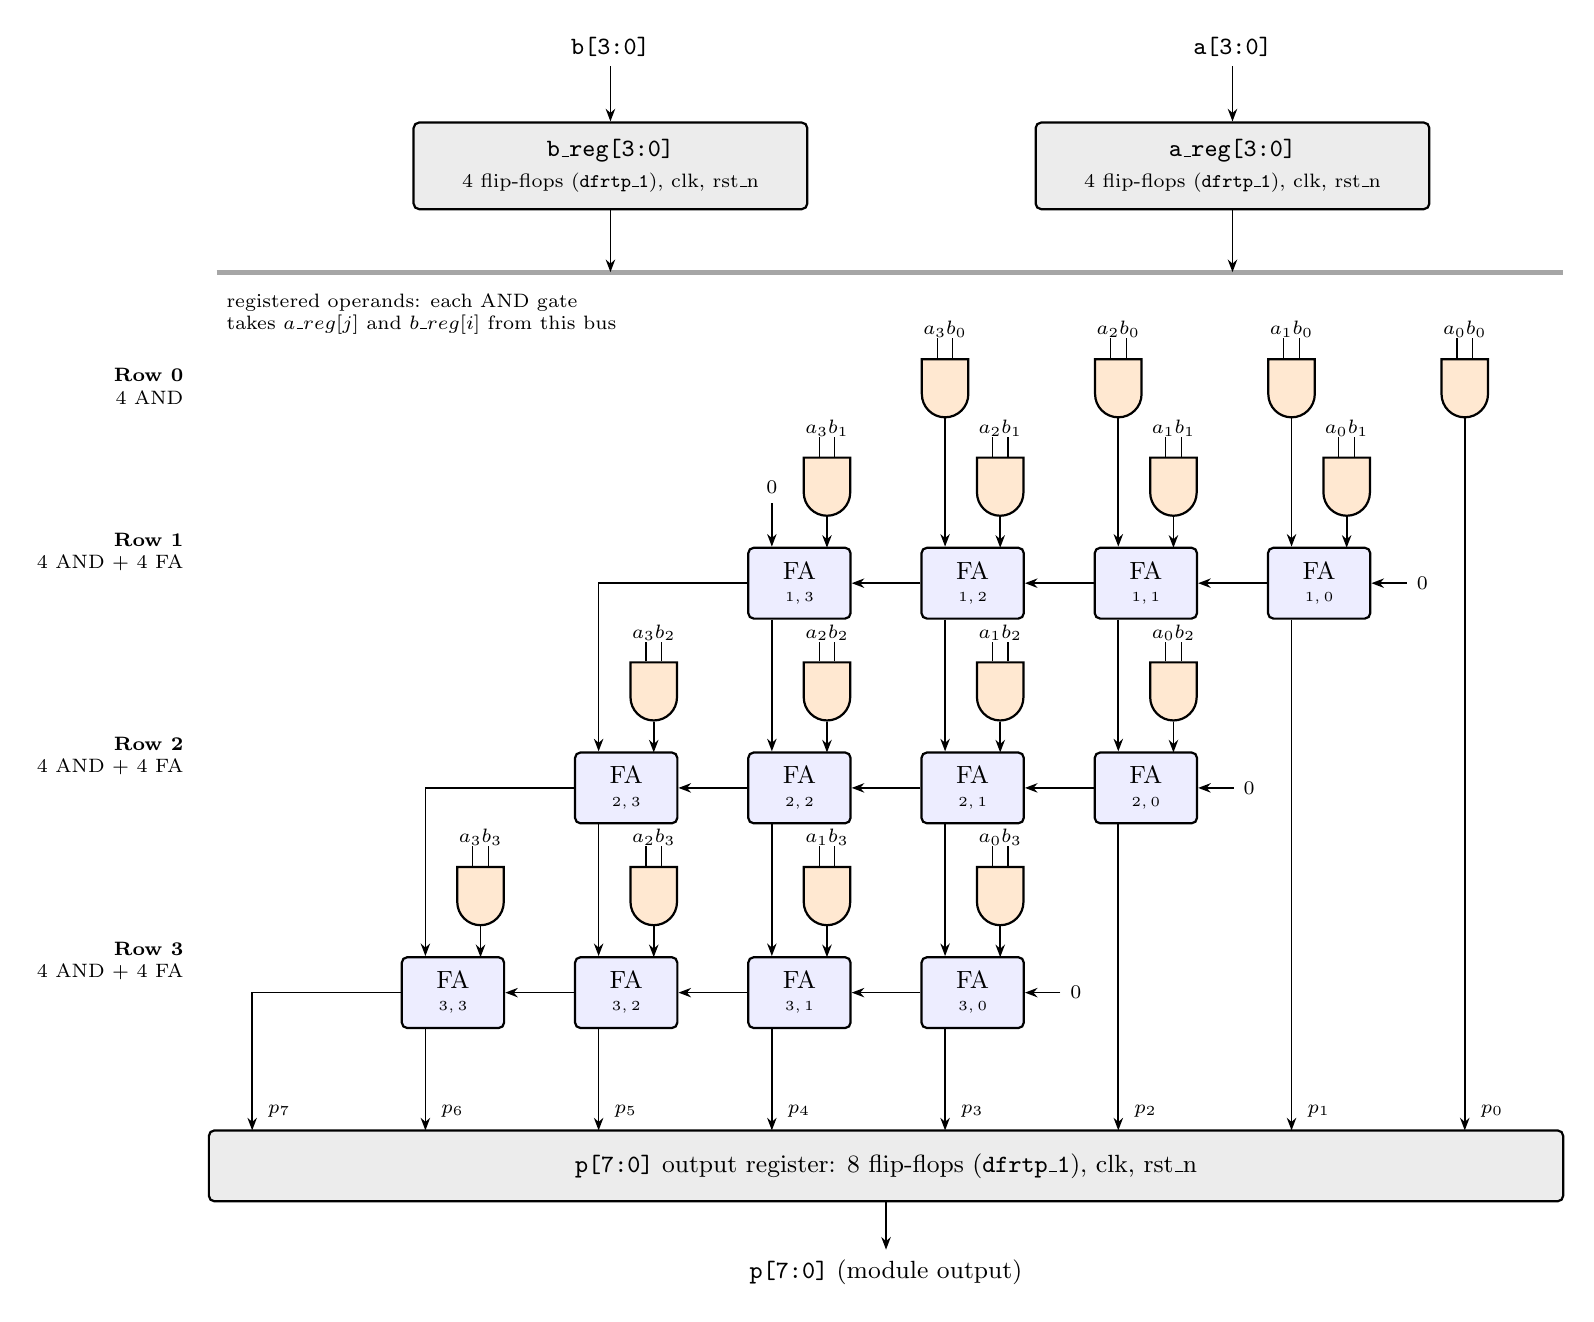
\begin{tikzpicture}[
  font=\small,
  fa/.style={draw, thick, rounded corners=2pt, minimum width=13mm, minimum height=9mm,
             fill=blue!7, align=center, inner sep=1pt},
  andg/.style={and gate US, draw, thick, logic gate inputs=nn, rotate=-90,
               minimum width=6mm, minimum height=5mm, fill=orange!18},
  w/.style={-{Stealth[length=1.6mm]}, semithick},
  reg/.style={draw, thick, fill=gray!15, align=center, rounded corners=2pt},
  lbl/.style={font=\scriptsize},
]
\def\dx{2.2}
\coordinate (bus) at (0, 2.45);
\coordinate (regtop) at (0, -8.45);

% Input registers and operand bus
\node[reg, minimum width=50mm, minimum height=11mm] (areg) at (12.1, 3.8)
  {\texttt{a\_reg[3:0]}\\\scriptsize 4 flip-flops (\cell{dfrtp\_1}), clk, rst\_n};
\node[reg, minimum width=50mm, minimum height=11mm] (breg) at (4.2, 3.8)
  {\texttt{b\_reg[3:0]}\\\scriptsize 4 flip-flops (\cell{dfrtp\_1}), clk, rst\_n};
\draw[w] ($(areg.north)+(0,0.7)$) node[above] {\texttt{a[3:0]}} -- (areg.north);
\draw[w] ($(breg.north)+(0,0.7)$) node[above] {\texttt{b[3:0]}} -- (breg.north);
\draw[line width=1.8pt, gray!70] (-0.8, 2.45) -- (16.3, 2.45);
\draw[w] (areg.south) -- (areg.south |- bus);
\draw[w] (breg.south) -- (breg.south |- bus);
\node[lbl, align=left, anchor=north west] at (-0.8, 2.3)
  {registered operands: each AND gate\\takes $a\_reg[j]$ and $b\_reg[i]$ from this bus};

% Row 0: four AND gates; columns are aligned by bit weight (weight 0 at right)
\foreach \j in {0,...,3} {
  \pgfmathsetmacro{\xx}{(7-\j)*\dx-0.35}
  \node[andg] (and-0-\j) at (\xx, 1.0) {};
  \draw (and-0-\j.input 1) -- ++(0,0.25);
  \draw (and-0-\j.input 2) -- ++(0,0.25);
  \node[lbl] at (\xx, 1.72) {$a_{\j}b_{0}$};
}

% Rows 1-3: four AND gates and four full adders each
\foreach \i/\yf in {1/-1.5, 2/-4.1, 3/-6.7} {
  \foreach \j in {0,...,3} {
    \pgfmathtruncatemacro{\k}{\i+\j}
    \pgfmathsetmacro{\xf}{(7-\k)*\dx}
    \pgfmathsetmacro{\xa}{\xf+0.35}
    \pgfmathsetmacro{\ya}{\yf+1.25}
    \node[fa] (fa-\i-\j) at (\xf, \yf) {FA\\[-3pt]\tiny $\i,\j$};
    \node[andg] (and-\i-\j) at (\xa, \ya) {};
    \draw (and-\i-\j.input 1) -- ++(0,0.25);
    \draw (and-\i-\j.input 2) -- ++(0,0.25);
    \node[lbl] at (\xa, \ya+0.72) {$a_{\j}b_{\i}$};
    \draw[w] (and-\i-\j.output) -- (\xa, \yf+0.45);
  }
}

% Ripple carries inside each row, carry-in of adder 0 tied to 0
\foreach \i in {1,2,3} {
  \foreach \j in {0,1,2} {
    \pgfmathtruncatemacro{\jn}{\j+1}
    \draw[w] (fa-\i-\j.west) -- (fa-\i-\jn.east);
  }
  \draw[w] ($(fa-\i-0.east)+(0.45,0)$) node[right, lbl] {0} -- (fa-\i-0.east);
}

% r0: row 0 passes pp0[3:1] down to row 1, top bit is 0
\foreach \j in {0,1,2} {
  \pgfmathtruncatemacro{\jn}{\j+1}
  \draw[w] (and-0-\jn.output) -- ($(fa-1-\j.north)+(-0.35,0)$);
}
\draw[w] ($(fa-1-3.north)+(-0.35,0.55)$) node[above, lbl] {0} -- ($(fa-1-3.north)+(-0.35,0)$);

% r1, r2: sums s[3:1] and the row carry-out pass down to the next row
\foreach \i in {2,3} {
  \pgfmathtruncatemacro{\ip}{\i-1}
  \foreach \j in {0,1,2} {
    \pgfmathtruncatemacro{\jn}{\j+1}
    \draw[w] ($(fa-\ip-\jn.south)+(-0.35,0)$) -- ($(fa-\i-\j.north)+(-0.35,0)$);
  }
  \draw[w] (fa-\ip-3.west) -| ($(fa-\i-3.north)+(-0.35,0)$);
}

% Finished product bits go down to the output register
\coordinate (o0) at (and-0-0.output);
\draw[w] (o0) -- (o0 |- regtop);
\foreach \i in {1,2,3} {
  \coordinate (o\i) at ($(fa-\i-0.south)+(-0.35,0)$);
  \draw[w] (o\i) -- (o\i |- regtop);
}
\foreach \j in {1,2,3} {
  \coordinate (q\j) at ($(fa-3-\j.south)+(-0.35,0)$);
  \draw[w] (q\j) -- (q\j |- regtop);
}
\draw[w] (fa-3-3.west) -| (-0.35, -8.45);

% Output register
\node[reg, minimum width=172mm, minimum height=9mm] (preg) at (7.7, -8.9)
  {\texttt{p[7:0]} output register: 8 flip-flops (\cell{dfrtp\_1}), clk, rst\_n};
\foreach \k in {0,...,7} {
  \pgfmathsetmacro{\xp}{(7-\k)*\dx-0.27}
  \node[lbl, anchor=west] at (\xp, -8.2) {$p_{\k}$};
}
\draw[w] (preg.south) -- ++(0,-0.6) node[below] {\texttt{p[7:0]} (module output)};

% Row labels
\node[lbl, align=right, anchor=east] at (-1.1, 1.0)  {\textbf{Row 0}\\4 AND};
\node[lbl, align=right, anchor=east] at (-1.1, -1.1) {\textbf{Row 1}\\4 AND + 4 FA};
\node[lbl, align=right, anchor=east] at (-1.1, -3.7) {\textbf{Row 2}\\4 AND + 4 FA};
\node[lbl, align=right, anchor=east] at (-1.1, -6.3) {\textbf{Row 3}\\4 AND + 4 FA};
\end{tikzpicture}}
\caption{Block diagram: 8 input flip-flops, 16 AND gates, 12 full adders (FA $i,j$
is adder $j$ of row $i$) and 8 output flip-flops. Columns are aligned by bit weight,
weight 0 on the right. Each FA takes the partial product from the AND gate above
it (right input) and the bit passed down from the previous row (left input); the
carry enters from the right and leaves to the left, and the sum leaves from the
bottom.}
\label{fig:block}
\end{figure}

\subsection{Testbench}

\texttt{tb/tb\_mult.v} is exhaustive and self-checking:
\begin{itemize}
  \item a 10~ns clock, with \texttt{rst\_n} held low for the first 2 cycles;
  \item all 256 combinations $a, b \in \{0 \ldots 15\}$, applied on the falling edge;
  \item for each one it waits the 2-cycle latency (two rising edges), then samples
        \texttt{p} on the next falling edge and compares it with \texttt{a * b}
        (the \texttt{*} operator appears only in the testbench);
  \item it prints a line for every mismatch, exactly one summary line at the end,
        and writes \texttt{mult.vcd}.
\end{itemize}
Sampling on the falling edge keeps the check away from the clock edge. This matters
for the gate-level simulation in Part B, where every cell has a unit delay and a
sample taken right after the rising edge would race with the flip-flop outputs.

\subsection{Results}

Simulation of the RTL:
\begin{Verbatim}[frame=single, fontsize=\small]
PASS: 256 vectors checked, 0 errors
\end{Verbatim}

\textbf{Error test (task 6).} \texttt{sum} in \texttt{full\_adder.v} was changed
from \texttt{a \^{} b \^{} cin} to \texttt{a \^{} b}; the testbench caught it (first
mismatches and the summary line shown), and the change was then undone:
\begin{Verbatim}[frame=single, fontsize=\small]
MISMATCH: a=3 b=3 expected=9 (00001001) got=5 (00000101) at time 1066000
MISMATCH: a=3 b=6 expected=18 (00010010) got=10 (00001010) at time 1126000
MISMATCH: a=3 b=7 expected=21 (00010101) got=9 (00001001) at time 1146000
FAIL: 256 vectors checked, 95 errors
\end{Verbatim}

\subsection{Worked example (task 5)}

$A$ = last digit of Neel Rajesh's roll number (2024102007) $+ 5 = 7 + 5 = 12$.
Since $A \neq 7$, $B = 7$. Expected product: $12 \times 7 = 84 = 0101\,0100_2$.

Worked in the same layout as the example in Section 2 of the assignment: one
partial product $pp_i = A \text{ AND } b_i$ per bit of $B$, shifted left by $i$,
then added.

\begin{table}[H]
\centering
\begin{tabular}{@{}*{8}{>{\ttfamily}c@{\hspace{5pt}}}@{\hspace{10pt}}l@{\hspace{14pt}}r@{}}
  & & & & 1 & 1 & 0 & 0 & $A$ & 12 \\
  & & & $\times$ & 0 & 1 & 1 & 1 & $B$ & 7 \\
\cline{2-8}
  & & & & 1 & 1 & 0 & 0 & $pp_0 = A$ AND $b_0$ ($b_0 = 1$) & 12 \\
  & & & 1 & 1 & 0 & 0 &   & $pp_1 = A$ AND $b_1$ ($b_1 = 1$), shifted 1 & 24 \\
  & & 1 & 1 & 0 & 0 & &   & $pp_2 = A$ AND $b_2$ ($b_2 = 1$), shifted 2 & 48 \\
  & 0 & 0 & 0 & 0 & & &   & $pp_3 = A$ AND $b_3$ ($b_3 = 0$), shifted 3 & 0 \\
\cline{1-8}
0 & 1 & 0 & 1 & 0 & 1 & 0 & 0 & $P = 12 + 24 + 48 + 0$ & \textbf{84} \\
\end{tabular}
\caption{Worked example $12 \times 7 = 84$.}
\label{tab:worked}
\end{table}

The same product traced through the array, row by row, using the connection
equations of Section 2 ($r_i$ is the 4-bit value row $i$ passes down;
$s_i$ and $c_i[4]$ are the sum bits and final carry of row $i$):

\begin{table}[H]
\centering
\small
\begin{tabular}{clllll}
\toprule
Row & $pp_i$ & Addition & Carry, sum & Product bit & Passes down \\
\midrule
0 & \texttt{1100} & AND gates only & -- & $p[0] = pp_0[0] = 0$ & $r_0 = \texttt{0110}$ \\
1 & \texttt{1100} & $pp_1 + r_0 = 12 + 6 = 18$ & $c_1[4] = 1$, $s_1 = \texttt{0010}$ & $p[1] = s_1[0] = 0$ & $r_1 = \texttt{1001}$ \\
2 & \texttt{1100} & $pp_2 + r_1 = 12 + 9 = 21$ & $c_2[4] = 1$, $s_2 = \texttt{0101}$ & $p[2] = s_2[0] = 1$ & $r_2 = \texttt{1010}$ \\
3 & \texttt{0000} & $pp_3 + r_2 = 0 + 10 = 10$ & $c_3[4] = 0$, $s_3 = \texttt{1010}$ & $p[3] = s_3[0] = 0$ & $p[7{:}4] = \texttt{0101}$ \\
\bottomrule
\end{tabular}
\caption{$12 \times 7$ through the array. Reading $p[7{:}4]$ and $p[3{:}0]$
together gives $p = \texttt{0101\,0100} = 84$.}
\label{tab:worked-array}
\end{table}

\begin{figure}[H]
\centering
\begin{tikzpicture}
  \node[anchor=south west, inner sep=0] (wf) at (0,0)
    {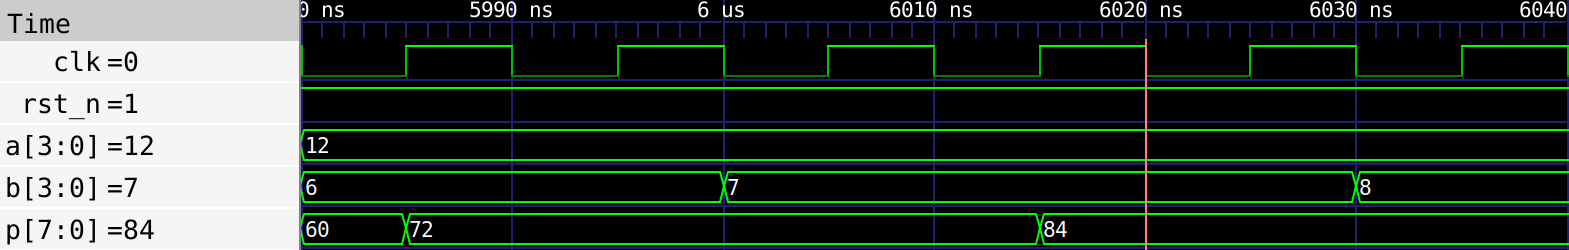
\includegraphics[width=\textwidth]{figures/waveform.png}};
  \begin{scope}[x={(wf.south east)}, y={(wf.north west)}]
    \draw[blue!70!black, thick, dotted] (0.4608,-0.08) -- (0.4608,1.08);
    \draw[red!75!black, very thick, dashed] (0.5271,-0.08) -- (0.5271,1.08);
    \draw[red!75!black, very thick, dashed] (0.6622,-0.08) -- (0.6622,1.08);
    \node[blue!70!black, font=\scriptsize, align=right, anchor=south east]
      at (0.4608,1.08) {6000 ns: $b$ changes to 7,\\inputs $12 \times 7$ applied};
    \node[red!75!black, font=\scriptsize\bfseries, align=right, anchor=north east]
      at (0.5271,-0.08) {edge 1 (6005 ns)\\$a, b$ captured into \texttt{a\_reg}, \texttt{b\_reg}};
    \node[red!75!black, font=\scriptsize\bfseries, align=left, anchor=north west]
      at (0.6622,-0.08) {edge 2 (6015 ns)\\product captured: $p = 84$};
  \end{scope}
\end{tikzpicture}
\caption{RTL waveform (GTKWave, 5980--6040 ns) for $12 \times 7$. The inputs
applied before edge 1 are captured at edge 1, and the product reaches \texttt{p}
at edge 2: a latency of 2 clock cycles. The GTKWave marker at 6020 ns, where the
testbench samples \texttt{p}, gives the values shown next to the signal names.}
\label{fig:wave}
\end{figure}

\begin{table}[H]
\centering
\small
\begin{tabular}{rllll}
\toprule
Time (ns) & Event & $a$ & $b$ & $p$ \\
\midrule
5985 & rising edge & 12 & 6 & 60 $\rightarrow$ 72 (result of $12 \times 6$) \\
6000 & new inputs applied (falling edge) & 12 & 7 & 72 \\
6005 & rising edge 1: inputs captured & 12 & 7 & 72 \\
6015 & rising edge 2: product captured & 12 & 7 & \textbf{84} \\
6030 & next inputs applied & 12 & 8 & 84 \\
\bottomrule
\end{tabular}
\caption{Values read from Figure~\ref{fig:wave}.}
\end{table}

% ---------------------------------------------------------------------------
\section{Part B: Logic Synthesis with Yosys}

\texttt{synth/synth.tcl} runs the seven required steps (\texttt{read\_verilog},
\texttt{synth -top mult\_array -flatten}, \texttt{dfflibmap}, \texttt{abc},
\texttt{opt\_clean -purge}, \texttt{stat}, \texttt{write\_verilog}) against the
typical-corner Liberty file.

\begin{table}[H]
\centering
\begin{tabular}{ll}
\toprule
Metric & Value \\
\midrule
Total number of cells & 67 \\
Number of flip-flops & 16 \\
Total cell area & 746.966~\umsq{} \\
Flip-flop area & 400.384~\umsq{} ($16 \times 25.024$) \\
Flip-flop area (\% of total) & 53.60\% \\
3 most-used cell types & \cell{dfrtp\_1} (16), \cell{nand2\_1} (12), \cell{xnor2\_1} (7) \\
Netlist simulation result & \texttt{PASS: 256 vectors checked, 0 errors} \\
\bottomrule
\end{tabular}
\caption{Part B results.}
\end{table}

\begin{table}[H]
\centering
\small
\begin{tabular}{lrr}
\toprule
Cell & Count & Area (\umsq) \\
\midrule
\cell{dfrtp\_1} & 16 & 400.384 \\
\cell{nand2\_1} & 12 & 45.043 \\
\cell{xnor2\_1} & 7 & 61.309 \\
\cell{a21oi\_1} & 4 & 20.019 \\
\cell{and2\_0} & 2 & 12.512 \\
\cell{lpflow\_isobufsrc\_1} & 2 & 12.512 \\
\cell{maj3\_1} & 2 & 20.019 \\
\cell{nand2b\_1} & 2 & 12.512 \\
\cell{nand4\_1} & 2 & 12.512 \\
\cell{nor3\_1} & 2 & 10.010 \\
\cell{o21a\_1} & 2 & 15.014 \\
\cell{o21ai\_0} & 2 & 10.010 \\
\bottomrule
\end{tabular}
\hspace{1cm}
\begin{tabular}{lrr}
\toprule
Cell & Count & Area (\umsq) \\
\midrule
\cell{xnor3\_1} & 2 & 45.043 \\
\cell{a21boi\_0} & 1 & 7.507 \\
\cell{a22oi\_1} & 1 & 7.507 \\
\cell{a32oi\_1} & 1 & 8.758 \\
\cell{and4\_1} & 1 & 8.758 \\
\cell{clkinv\_1} & 1 & 3.754 \\
\cell{nand3\_1} & 1 & 5.005 \\
\cell{nor2\_1} & 1 & 3.754 \\
\cell{o21ba\_1} & 1 & 10.010 \\
\cell{or3\_1} & 1 & 6.256 \\
\cell{xor2\_1} & 1 & 8.758 \\
\midrule
\textbf{Total} & \textbf{67} & \textbf{746.966} \\
\bottomrule
\end{tabular}
\caption{All cells in the synthesised netlist (\texttt{synth/mult\_array\_stat.rpt}).}
\end{table}

The synthesised netlist was simulated with the same testbench, using the SKY130
cell models with \texttt{-DFUNCTIONAL -DUNIT\_DELAY=\#1}, and printed
\texttt{PASS: 256 vectors checked, 0 errors}, so synthesis did not change the
behaviour.

% ---------------------------------------------------------------------------
\section{Part C: Static Timing Analysis with OpenSTA}

\texttt{sta/sta.tcl} reads the typical-corner Liberty file and the netlist, defines
the clock, sets 1.0~ns input and output delays, and reports the worst setup slack
and the critical path. At $T = 10$~ns the worst slack was 7.396~ns, so
\[
T_{min} = 10 - 7.396 = 2.604~\text{ns}, \qquad
F_{max} = \frac{1000}{2.604} = 384.0~\text{MHz}.
\]
Re-running at $T = 2.60$~ns gave a slack of $-0.004$~ns, close to 0, which confirms
the calculation.

\begin{table}[H]
\centering
\begin{tabular}{ll}
\toprule
Metric & Value \\
\midrule
Worst slack at $T = 10$~ns & 7.396~ns \\
$T_{min}$ & 2.604~ns \\
$F_{max}$ & 384.0~MHz \\
Slack at $T = T_{min}$ (2.60~ns) & $-0.004$~ns ($\approx 0$) \\
Critical path start point & \texttt{\_106\_} (\cell{dfrtp\_1}, \texttt{b\_reg[0]}) \\
Critical path end point & \texttt{\_100\_} (\cell{dfrtp\_1}, \texttt{p[6]}) \\
Cells on the critical path & 8 combinational (10 including both flip-flops) \\
Latency $= 2 \times T_{min}$ & 5.208~ns \\
Throughput & 384.0 million results per second \\
\bottomrule
\end{tabular}
\caption{Part C results.}
\end{table}

\begin{table}[H]
\centering
\small
\begin{tabular}{lllrrl}
\toprule
\# & Instance & Cell & Delay (ns) & Arrival (ns) & Function \\
\midrule
-- & \texttt{\_106\_} & \cell{dfrtp\_1} & 0.388 & 0.388 & launch flip-flop \texttt{b\_reg[0]} (clock to Q) \\
1 & \texttt{\_043\_} & \cell{and2\_0}  & 0.180 & 0.568 & partial product (AND) \\
2 & \texttt{\_056\_} & \cell{or3\_1}   & 0.391 & 0.959 & carry logic merged by ABC \\
3 & \texttt{\_058\_} & \cell{a32oi\_1} & 0.250 & 1.208 & partial products merged into carry logic \\
4 & \texttt{\_072\_} & \cell{o21ba\_1} & 0.198 & 1.406 & carry logic merged by ABC \\
5 & \texttt{\_073\_} & \cell{xnor2\_1} & 0.147 & 1.553 & adder sum \\
6 & \texttt{\_082\_} & \cell{maj3\_1}  & 0.385 & 1.937 & full-adder carry (majority) \\
7 & \texttt{\_084\_} & \cell{maj3\_1}  & 0.358 & 2.295 & full-adder carry (majority) \\
8 & \texttt{\_088\_} & \cell{xnor3\_1} & 0.175 & 2.471 & full-adder sum, drives \texttt{p\_next[6]} \\
-- & \texttt{\_100\_} & \cell{dfrtp\_1} & setup 0.134 & -- & capture flip-flop \texttt{p[6]} \\
\bottomrule
\end{tabular}
\caption{Critical path at $T = 2.60$~ns (\texttt{sta/mult\_array\_timing.rpt}).}
\end{table}

\textbf{Cells from full adders (task 3).} Four of the eight combinational cells are
plain full-adder functions: two \cell{maj3\_1} carries, one \cell{xnor3\_1} sum and
one \cell{xnor2\_1} sum. One, \cell{and2\_0}, is a partial-product AND gate. The
other three (\cell{or3\_1}, \cell{a32oi\_1}, \cell{o21ba\_1}) are compound cells in
which ABC merged partial-product ANDs into the carry logic. Section 2 estimates the
longest path as about $2N = 8$ full-adder delays. The path does have 8 cells, but
each one is a single library cell, not a full adder built from two gate levels
(see question 2).

% ---------------------------------------------------------------------------
\section{Part D: Physical Design with LibreLane}

\begin{table}[H]
\centering
\begin{tabular}{ll}
\toprule
Key & Value \\
\midrule
\texttt{DESIGN\_NAME} & \texttt{"mult\_array"} \\
\texttt{VERILOG\_FILES} & \texttt{["dir::../rtl/full\_adder.v", "dir::../rtl/mult\_array.v"]} \\
\texttt{CLOCK\_PORT} & \texttt{"clk"} \\
\texttt{CLOCK\_PERIOD} & 3.5 \ ($1.2 \times T_{min} = 1.2 \times 2.604 = 3.125$, rounded up to the next 0.5~ns) \\
\texttt{FP\_SIZING} & \texttt{"absolute"} \\
\texttt{DIE\_AREA} & \texttt{[0, 0, 150, 150]} \\
\bottomrule
\end{tabular}
\caption{\texttt{pnr/config.json}.}
\end{table}

The first run (\texttt{RUN\_2026-10-25\_10-24-37}) finished with 0 DRC, 0 LVS and
0 antenna errors and positive setup slack, so no further runs were needed.
\texttt{final/metrics.json} and \texttt{final/gds/mult\_array.gds} were copied
into \texttt{pnr/}.

\begin{table}[H]
\centering
\begin{tabular}{ll}
\toprule
Metric & Value \\
\midrule
\texttt{CLOCK\_PERIOD} used & 3.5~ns \\
Number of runs needed & 1 \\
Core area & 17\,759.5~\umsq{} (die $150 \times 150 = 22\,500$~\umsq) \\
Cells after synthesis (Part B) & 67 \\
Cells after place and route & 1886 \\
Kinds of cells added & decap, fill, tap, I/O buffers, clock buffers, timing-repair buffers \\
Wirelength & 2381~\um{} \\
Setup slack & $+0.605$~ns (typical corner, \texttt{nom\_tt\_025C\_1v80}) \\
Post-route $F_{max}$ & $1000 / (3.5 - 0.605) = 345.4$~MHz \\
$F_{max}$ from Part C & 384.0~MHz \\
DRC errors & 0 (Magic 0, KLayout 0) \\
LVS errors & 0 \\
\bottomrule
\end{tabular}
\caption{Part D results (\texttt{pnr/metrics.json}).}
\end{table}

\begin{table}[H]
\centering
\small
\begin{tabular}{llr}
\toprule
Kind & Cells (instance names) & Count \\
\midrule
Decap & \cell{decap\_3}, \cell{decap\_4}, \cell{decap\_6}, \cell{decap\_8}, \cell{decap\_12} & 1292 \\
Fill & \cell{fill\_1}, \cell{fill\_2} & 258 \\
Tap & \cell{tapvpwrvgnd\_1} & 245 \\
Input/output buffers & \cell{buf\_2} (\texttt{input1}--\texttt{input9}, \texttt{output10}--\texttt{output17}) & 17 \\
Clock tree buffers & \cell{clkbuf\_16} & 3 \\
Setup-repair buffers & \cell{buf\_4} (\texttt{rebuffer*}) & 5 \\
Hold-fix delay cells & \cell{dlygate4sd3\_1} (\texttt{hold*}) & 3 \\
Fanout buffers & \cell{clkdlybuf4s50\_1} (\texttt{fanout*}) & 2 \\
Logic & & 45 \\
Flip-flops & \cell{dfrtp\_1} & 16 \\
\midrule
\textbf{Total} & & \textbf{1886} \\
\bottomrule
\end{tabular}
\caption{Where the 1886 cells come from (\texttt{metrics.json} and the final
netlist). LibreLane runs its own Yosys synthesis from the RTL, which is why the
logic is 45 cells here and 51 in Part B.}
\label{tab:added}
\end{table}

\textbf{Timing corner.} Parts B and C use the typical corner, so the slack quoted
above is the typical-corner value, which keeps the comparison with Part C like for
like. LibreLane also analyses fast and slow corners. All fast and typical corners
pass setup; the slow corner (\texttt{ss\_100C\_1v60}, 1.60~V and 100\,$^\circ$C)
does not. The all-corner \texttt{timing\_\_setup\_\_ws} in \texttt{metrics.json}
is $-2.118$~ns, with 5 violations in each slow corner. Hold slack is positive at
all nine corners (worst $+0.104$~ns).

\begin{figure}[H]
\centering
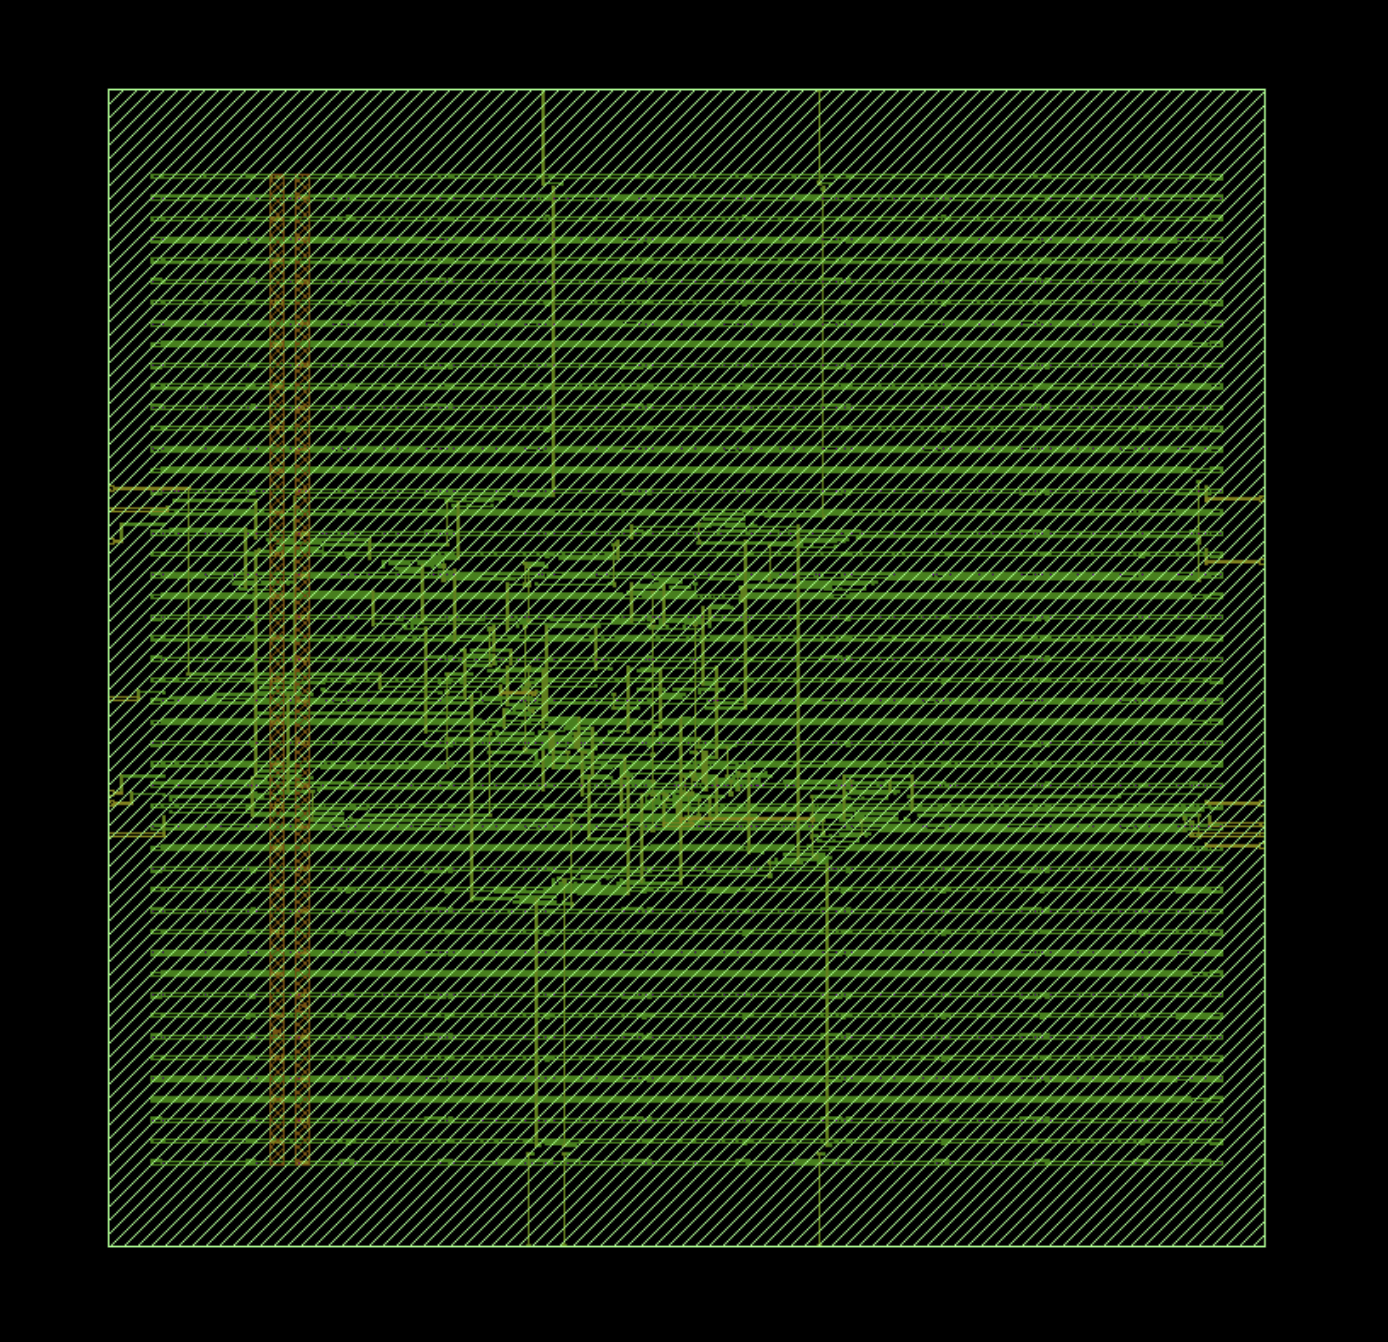
\includegraphics[width=0.72\textwidth]{figures/layout.png}
\caption{Whole die in KLayout, metal layers 1--4 only. The horizontal lines are
the metal-1 power rails, one per standard-cell row; the vertical pair on the left
is a metal-4 power strap. The signal routing is concentrated in the centre, where
the multiplier logic sits, with wires running out to the pins on the left and
right edges.}
\label{fig:die}
\end{figure}

\begin{figure}[H]
\centering
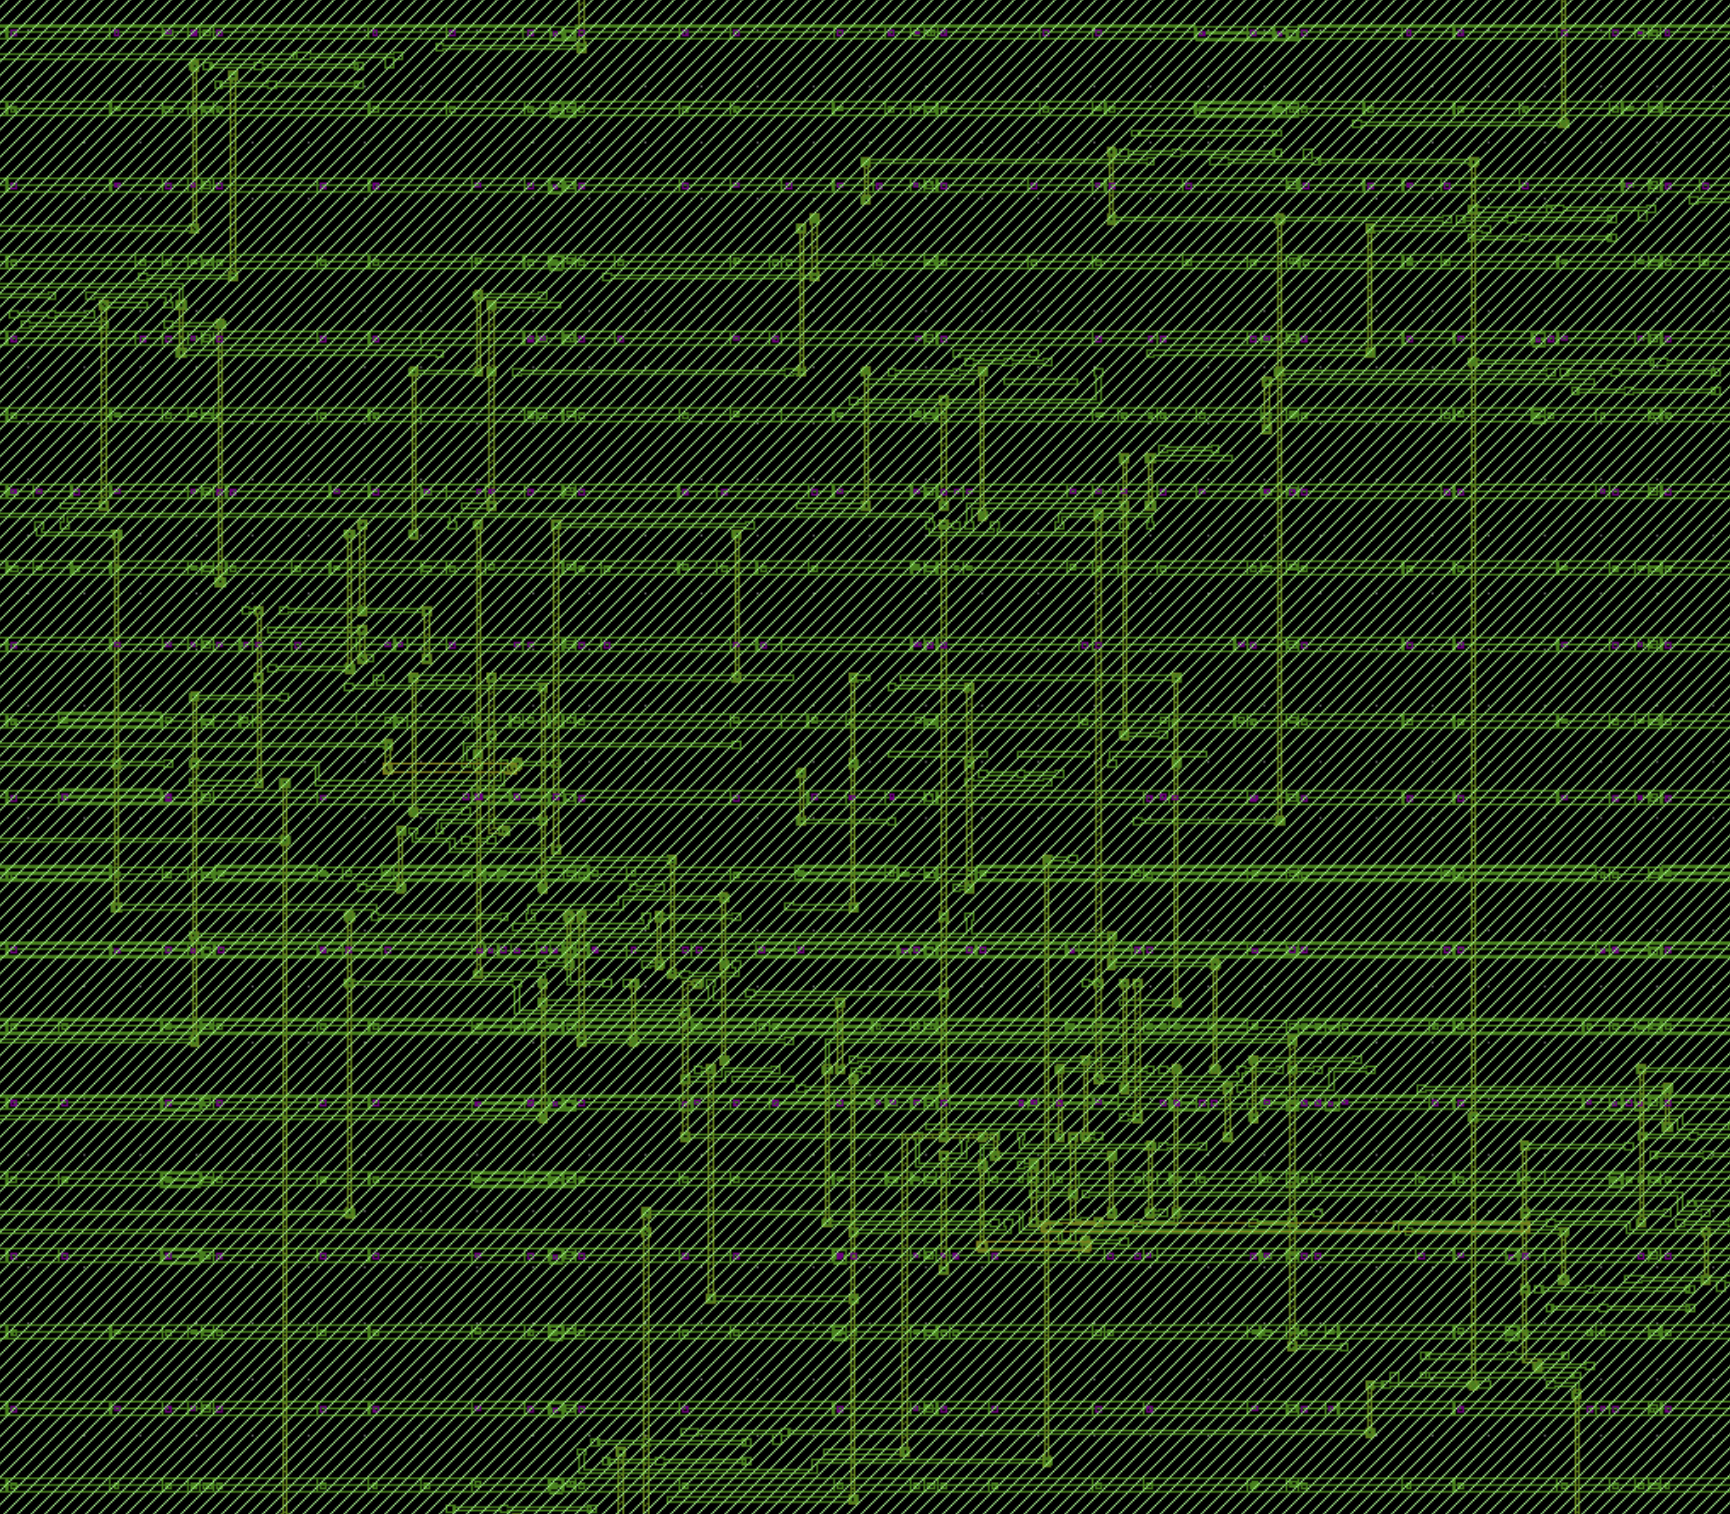
\includegraphics[width=0.78\textwidth]{figures/layout_zoomed.png}
\caption{Zoomed view of the centre of the die, metal layers only. Each horizontal
line is a metal-1 power rail along a standard-cell row; the wires between them are
the signal routing on metal 1--3.}
\label{fig:zoom}
\end{figure}

% ---------------------------------------------------------------------------
\section{Answers to the Questions}

\subsection*{1. Logic cells versus 16 AND gates + 12 full adders}

Synthesis produced 67 cells, of which 16 are flip-flops, so $67 - 16 = 51$ cells
implement the logic, against the $16 + 12 = 28$ components in the RTL. The numbers
differ because synthesis does not keep the RTL structure; it maps the Boolean
functions of the whole flattened array onto the cells in the library:
\begin{itemize}
  \item \textbf{A full adder is not one cell.} SKY130 has a full-adder cell, but it
        has two outputs, and ABC maps single-output functions only. So each sum
        and each carry is built separately: the sums from XOR/XNOR cells
        (7 \cell{xnor2\_1}, 2 \cell{xnor3\_1}, 1 \cell{xor2\_1}), the carries from
        majority and AND-OR-invert cells (2 \cell{maj3\_1}, plus \cell{a21oi},
        \cell{a22oi}, \cell{a32oi}, \cell{o21a}, \cell{o21ai} and others).
  \item \textbf{The AND gates mostly disappear.} Only 2 \cell{and2\_0} and one
        \cell{and4\_1} remain; the other partial products are absorbed into the 12
        \cell{nand2\_1} cells and into compound AOI/OAI cells.
  \item \textbf{Constants simplify the array.} $c_1[0] = c_2[0] = c_3[0] = 0$ and
        $r_0[3] = 0$ turn four of the full adders into half adders, and Yosys
        removed the constant top bit of $r_0$ (\texttt{WREDUCE: Removed top 1 bits
        (of 4) from wire mult\_array.r0}).
  \item \textbf{Polarity fixes.} A few cells (\cell{clkinv\_1}, \cell{nand2b\_1},
        \cell{lpflow\_isobufsrc\_1}) exist only to invert or gate signals so that
        the inverting cells above can be used.
\end{itemize}

\subsection*{2. Critical path}

The critical path runs from flip-flop \texttt{\_106\_} (\texttt{b\_reg[0]}) to
flip-flop \texttt{\_100\_} (\texttt{p[6]}), through 8 combinational cells (10
including the two flip-flops), with 2.083~ns of logic delay after the 0.388~ns
clock-to-Q. Its shape matches what Section 2 predicts: it starts at an operand
bit that feeds the first rows and ripples through the carry chains down to a high
product bit. Section 2 estimates about $2N = 8$ full-adder delays. The path does
have 8 cells, but they are not 8 full adders: only 4 are plain full-adder
functions (two \cell{maj3\_1} carries, one \cell{xnor3\_1} and one \cell{xnor2\_1}
sum), one is a partial-product AND, and three are compound cells in which ABC
merged ANDs into the carry logic. Because SKY130 has one-cell majority and
three-input XNOR gates, a full-adder carry or sum costs one cell (about 0.26~ns on
average here) instead of two gate levels. ABC also restructured the logic across
row boundaries, so the real path is shorter than 8 two-level full adders would be.

\subsection*{3. Flip-flop share of the area}

Flip-flops take 400.384 of 746.966~\umsq, which is \textbf{53.60\%}. A
\cell{dfrtp\_1} is 25.024~\umsq, 6.7 times a \cell{nand2\_1} (3.754~\umsq). It is a
master-slave flip-flop with an asynchronous reset: the LVS report shows 28
transistors for \cell{dfrtp\_1} against 4 for \cell{nand2\_1}. The design needs 16
of them (4 + 4 input bits and 8 output bits), while the arithmetic is only 51 small
gates. Register count grows linearly with the width ($4N$) but the array grows
with $N^2$, so in a multiplier this small the registers dominate. At $N = 8$ the
array would be about 4.7 times larger (56 instead of 12 full adders) while the
registers would only double, so the flip-flop share would drop.

\subsection*{4. Why post-route $F_{max}$ is lower, and the added cells}

Post-route $F_{max}$ is $1000 / (3.5 - 0.605) = 1000 / 2.895 = 345.4$~MHz, 10\%
below the 384.0~MHz of Part C. Part C timed an unplaced netlist with an ideal clock
(zero delay and zero skew), no extracted wire parasitics and no margin. Post-route timing uses
the extracted wire resistance and capacitance, the real clock tree, the buffers the
flow inserted, and LibreLane's own constraints. Both analyses report the same
critical path, \texttt{b\_reg[0]} $\rightarrow$ \texttt{p[6]}, so the difference
in minimum period ($2.895 - 2.604 = 0.291$~ns) can be split exactly:

\begin{table}[H]
\centering
\small
\begin{tabularx}{\textwidth}{Yr}
\toprule
Contribution & ns \\
\midrule
Clock uncertainty: LibreLane's constraints reserve 0.25~ns for clock jitter; Part C had none & $+0.250$ \\
Data path, clock-to-Q to D: 2.522 vs 2.471~ns (real wire load, two inserted \cell{buf\_4} rebuffers, different logic from LibreLane's synthesis) & $+0.051$ \\
Clock tree: the launch clock arrives 0.030~ns later than the capture clock, offset by 0.031~ns of common-path pessimism removal & $-0.001$ \\
Setup time of the capture flip-flop: 0.124 vs 0.134~ns & $-0.010$ \\
\midrule
Total (difference from rounding) & $+0.290$ \\
\bottomrule
\end{tabularx}
\end{table}

So in this design most of the loss is the clock-uncertainty margin. The physical
effects add only about 0.05~ns, because the wires are short: 2381~\um{} in total,
and the longest net is 151~\um. In a larger design, wire delay would be a much
bigger share.

The flow added these kinds of cells (Table~\ref{tab:added}):
\begin{itemize}
  \item \textbf{Decap (1292):} capacitors between the supply rails that deliver
        charge locally when many cells switch at once, reducing supply droop and
        noise.
  \item \textbf{Fill (258):} close the gaps in each row so that the wells, implants
        and power rails are continuous, which the manufacturing (DRC and density)
        rules require.
  \item \textbf{Tap (245):} connect the n-well to VPWR and the substrate to VGND at
        regular intervals to prevent latch-up; \texttt{sky130\_fd\_sc\_hd} cells have
        no taps of their own.
  \item \textbf{Input/output buffers (17):} one on each input pin except the clock
        and one on each output, isolating the internal logic from external loads and
        drivers.
  \item \textbf{Clock tree buffers (3):} clock tree synthesis distributes
        \texttt{clk} to all 16 flip-flops with small skew and clean edges.
  \item \textbf{Setup-repair buffers (5):} the resizer splits and strengthens slow,
        heavily loaded nets. Two of them are on the critical path.
  \item \textbf{Hold-fix delay cells (3):} the shortest paths, \texttt{a\_reg[0]}
        and \texttt{b\_reg[0]} through a single AND gate to \texttt{p[0]}, would
        change too soon after the clock edge, so delay cells were added to them.
  \item \textbf{Fanout buffers (2):} \texttt{rst\_n} drives all 16 flip-flop resets,
        so it was split into two nets driving 10 and 6 flip-flops.
\end{itemize}

\subsection*{5. DRC and LVS}

\textbf{DRC} (design rule check) verifies that the layout geometry obeys the
foundry's manufacturing rules: minimum widths, spacings, enclosures and densities
on every layer. \textbf{LVS} (layout versus schematic) extracts the circuit from
the layout and checks that it is the same circuit as the intended netlist: the same
devices, connected in the same way. For our layout, Magic and KLayout both reported
0 DRC errors; for LVS, both netlists contained 1886 cell instances and 103 nets, and
Netgen reported \emph{Circuits match uniquely}. Both must pass because each catches
what the other cannot. A DRC-clean layout can still be the wrong circuit (a
misconnected or missing wire), and an LVS-clean layout can still be unmanufacturable
(shapes too close together become shorts, or too thin become opens, on silicon).
Only a layout that passes both is both buildable and correct.

\subsection*{6. Scaling to 8 bits}

Using the formulas in Section 2 with $N = 8$ instead of $N = 4$:
\begin{align*}
\text{AND gates: } & N^2 = 16 \;\rightarrow\; 64 \quad (4\times)\\
\text{Full adders: } & N(N-1) = 4 \times 3 = 12 \;\rightarrow\; 8 \times 7 = 56 \quad (4.7\times)\\
\text{Critical path: } & 2N = 8 \;\rightarrow\; 16 \text{ full-adder delays} \quad (2\times)\\
\text{Flip-flops: } & 4N = 16 \;\rightarrow\; 32 \quad (2\times)
\end{align*}
Our 4-bit path has 2.083~ns of logic for 8 full-adder delays, about 0.26~ns each.
For 8 bits:
\[
T_{min} \approx 16 \times 0.26 + 0.388 + 0.134 = 4.17 + 0.52 = 4.69~\text{ns},
\qquad F_{max} \approx \frac{1000}{4.69} \approx 213~\text{MHz}.
\]
The full-adder count grows with $N^2$ but the delay only with $N$: doubling the
width roughly quadruples the logic and doubles the critical-path delay, so
$F_{max}$ falls from 384~MHz to about 213~MHz.

\end{document}
